\section{Durchführung}
\label{sec:Durchführung}

\begin{figure}
    \centering
    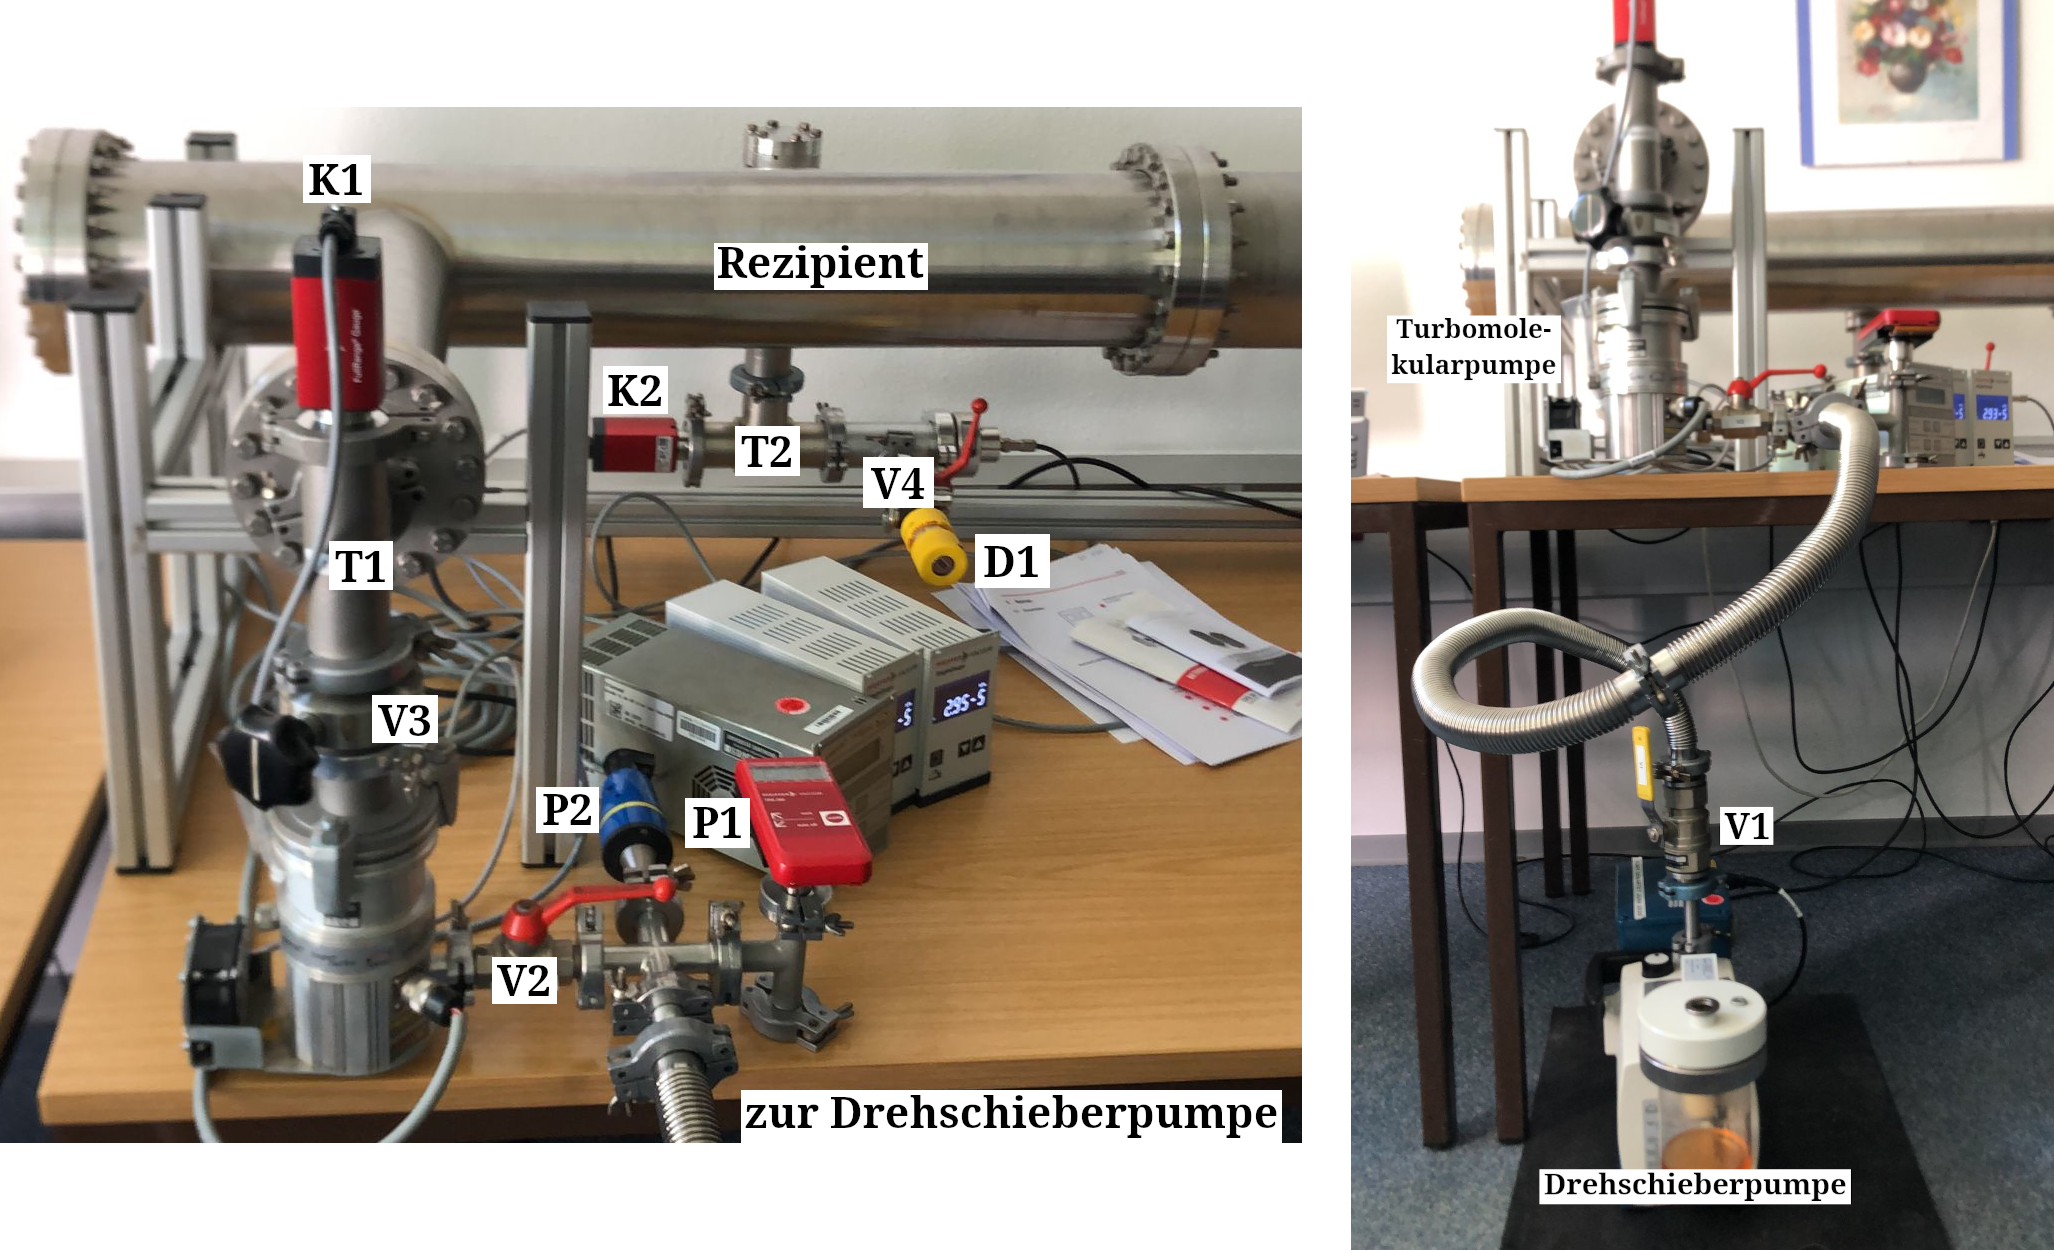
\includegraphics[width=0.8\textwidth]{abb/Aufbau.png}
    \caption{Aufbau des Versuches}
    \label{fig:Aufbau}
\end{figure}

Der Aufbau des Experimentes ist der \autoref{fig:Aufbau} zu entnehmen. Anfänglich lief die gesamte Apperatur etwas mehr als eine Stunde um einen Enddruck festzustellen.

\subsection{Drehschieberpumpe}
Die Evakuierungskurve der Drehschieberpumpe wurde aufgenommen, indem durch das Dosierventil D1 und Belüftungsventil V3, die mit dem kombinierten Pirani/Kaltkathoden-Sensor K2
am T-Rohr T2 angebracht sind, der Rezipient auf einen Normaldruck von \SI{1000}{\milli\bar} gebracht wurde. 
Nach anschließendem Verschließen von V3 wird der Druckabfall durch den kombinierten Piezo/Pirani-Sensor P1, der am Kreuzbauteil zwische
Drehschieber- und Turbomolekularpumpe angeschlossen ist, in Abhängigkeit von der Zeit gemessen.
Dabei liegen die Messintervalle bei \SI{10}{\second} und die Gesamtdauer bei \SI{600}{\second}. Diese Messung wird 3-mal wiederholt. Während dieser Messreihe
läuft ausschließlich die Drehschieberpumpe und Ventile V1 und V2 sind offen.

Bei der Leckratenmessung wird V3 wieder geöffnet und ein Gleichgewichtsdruck $p_g$ durch D1 hergestellt. Anschließend wird das Ventil V1 geschlossen, welches sich direkt hinter der
Drehschieberpumpe befindet. V2 bleibt weiterhin offen. Somit wird ein Druckanstieg hervorgerufen, der wieder durch P1 gemessen wird. Ein einzelnes Messintervall bleibt bei \SI{10}{\second},
jedoch verkürzt sich die Gesamtdauer auf lediglich \SI{200}{\second}. Diese Messung wird 3-mal wiederholt für 4 verschiedene $p_g$.

\subsection{Turbomolekularpumpe}
Zur Inbetriebnahme der Turbomolekularpumpe muss ein Vorkauum durch die Drehschieberpumpe erzeugt werden, das unter \SI{0.1}{\milli\bar} liegt. Die Drehzahlbegrenzung beträgt \SI{1350}{\hertz}.

Das Messverfahren der Turbopumpe wird analog zur Drehschieberpumpe durchgeführt. Lediglich die Konstellation der einzelnen Ventile und Messgeräte ändert sich.
Der Druck wird durch Ablesen des Anzeigegerätes des komibinierten Pirani/Kaltkathoden-Sensors K1, der hinter der Pumpe am T-Rohr T1 angebracht ist, abgelesen.

Die Evakuierungskurve wird wieder 3-mal während laufender Turbopumpe aufgenommen. Die Gesamtdauer der Messung verändert sich dabei zu \SI{120}{\second}. Dahingegen bleiben die Messintervalle gleich.
Diese Änderung wird auch in der Leckratenmessung vorgenommen, bei der durch Schließen des Ventils V2 ein Druckanstieg verursacht wird.